\section*{Problem 2}

Compute the DTFT of the following signals and sketch $X(\omega)$.

\begin{itemize}
\item 
$x[n] =
\left[
\begin{array}{c c c c}
 \frac{1}{4}&  \frac{1}{4}& \frac{1}{4}& \frac{1}{4}
 \end{array}
 \right]
$
\end{itemize} 

\subsection*{Solution}

Aplying the definition of (\ref{eq:c41}) we have:

\begin{equation*}
\begin{aligned}
X(\omega) &= \displaystyle\sum_{0}^{3} \frac{1}{4} e^{-j \omega n} \\
&= \frac{1}{4} [1 + e^{-jw} + e^{-2jw} + e^{-3jw}] \\
&= \frac{1}{4} e^{-j \frac{3 \omega}{2}}
		[e^{j \frac{3 \omega}{2}} + e^{-j \frac{\omega}{2}} + 
		 e^{- j \frac{\omega}{2}} + e^{-j \frac{3 \omega}{2}} ] \\
&= \frac{1}{2}  e^{-j \frac{3 \omega}{2}} [\cos(\frac{3 \omega}{2})\cos(\frac{\omega}{2})]
\end{aligned}
\end{equation*} 

The plot of the magintude $X(\omega)$ is:
\zcodemat{sources/c4p1a.m}{Plot of Magnitude}

\begin{figure}[H]
\caption{Magnitude $|X(\omega)|$}
\centering
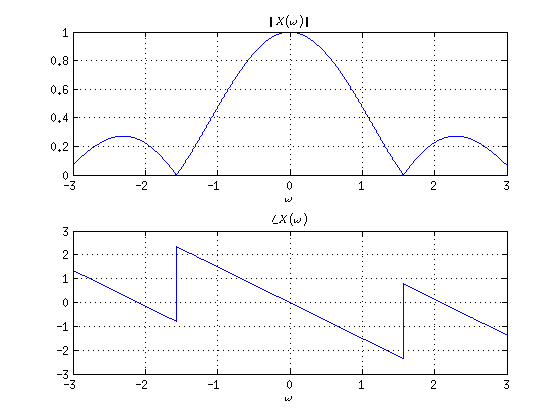
\includegraphics[width=1.0\textwidth]{figs/c4p1a.png}
\label{fig:c4p1a}
\end{figure} 

